\documentclass[titlepage, 12pt]{article}

\usepackage{framed}
\usepackage{enumitem}
\usepackage{geometry}
\geometry{
  letterpaper,
  margin=1in,
}

\usepackage{graphicx}
\graphicspath{{./images/}}
\usepackage{hyperref}
\usepackage{float}
% \usepackage{subcaption}
\usepackage{amssymb}

\title{SE 2XB3 Group 4 Report 7}
\author{
  Huang, Kehao \\
  400235182 \\
  \texttt{huangk53@mcmaster.ca} \\
  L01
  \and
  Jiao, Anhao \\
  400251837 \\
  \texttt{jiaoa3@mcmaster.ca} \\
  L01
  \and
  Ye, Xunzhou \\
  400268576 \\
  \texttt{yex33@mcmaster.ca} \\
  L01
}
\date{12 March 2021}

\begin{document}
\maketitle{}

\newpage{}

\section{Cycles and Connected Probability}

For the experiment, we added edge \(a \rightarrow b\) by randomly choosing
\(a, b\) over the interval \(0 \leq a, b < k\). We experimented with different
\(c\) values ranged from 1 to \(3k = 300\). For each of the \(c\) values, 10
graphs with randomly added edges were tested about its cyclic property and
connected property. The portions are calculated based of the 10 samples taken
for each \(c\) value. Figure \ref{fig:cyclic} and Figure \ref{fig:connect} are
the results of our experiments. For \(c \approx 60\), roughly half the graphs
contained a cycle, and for \(c \approx 250\), roughly half the graphs are
connected. The \(c\) value for graphs to be connected being much less than the
other is reasonable because the minimum number of edges required to form a cycle
is 3 while the minimum for forming a connected graph of size \(k\) is \(k - 1\).
Due to the fact that all the graphs tested in the experiment were of size 100,
for any graph to be fully connected is obviously less likely than it being cyclic.

\begin{figure}[h]
  \centering
  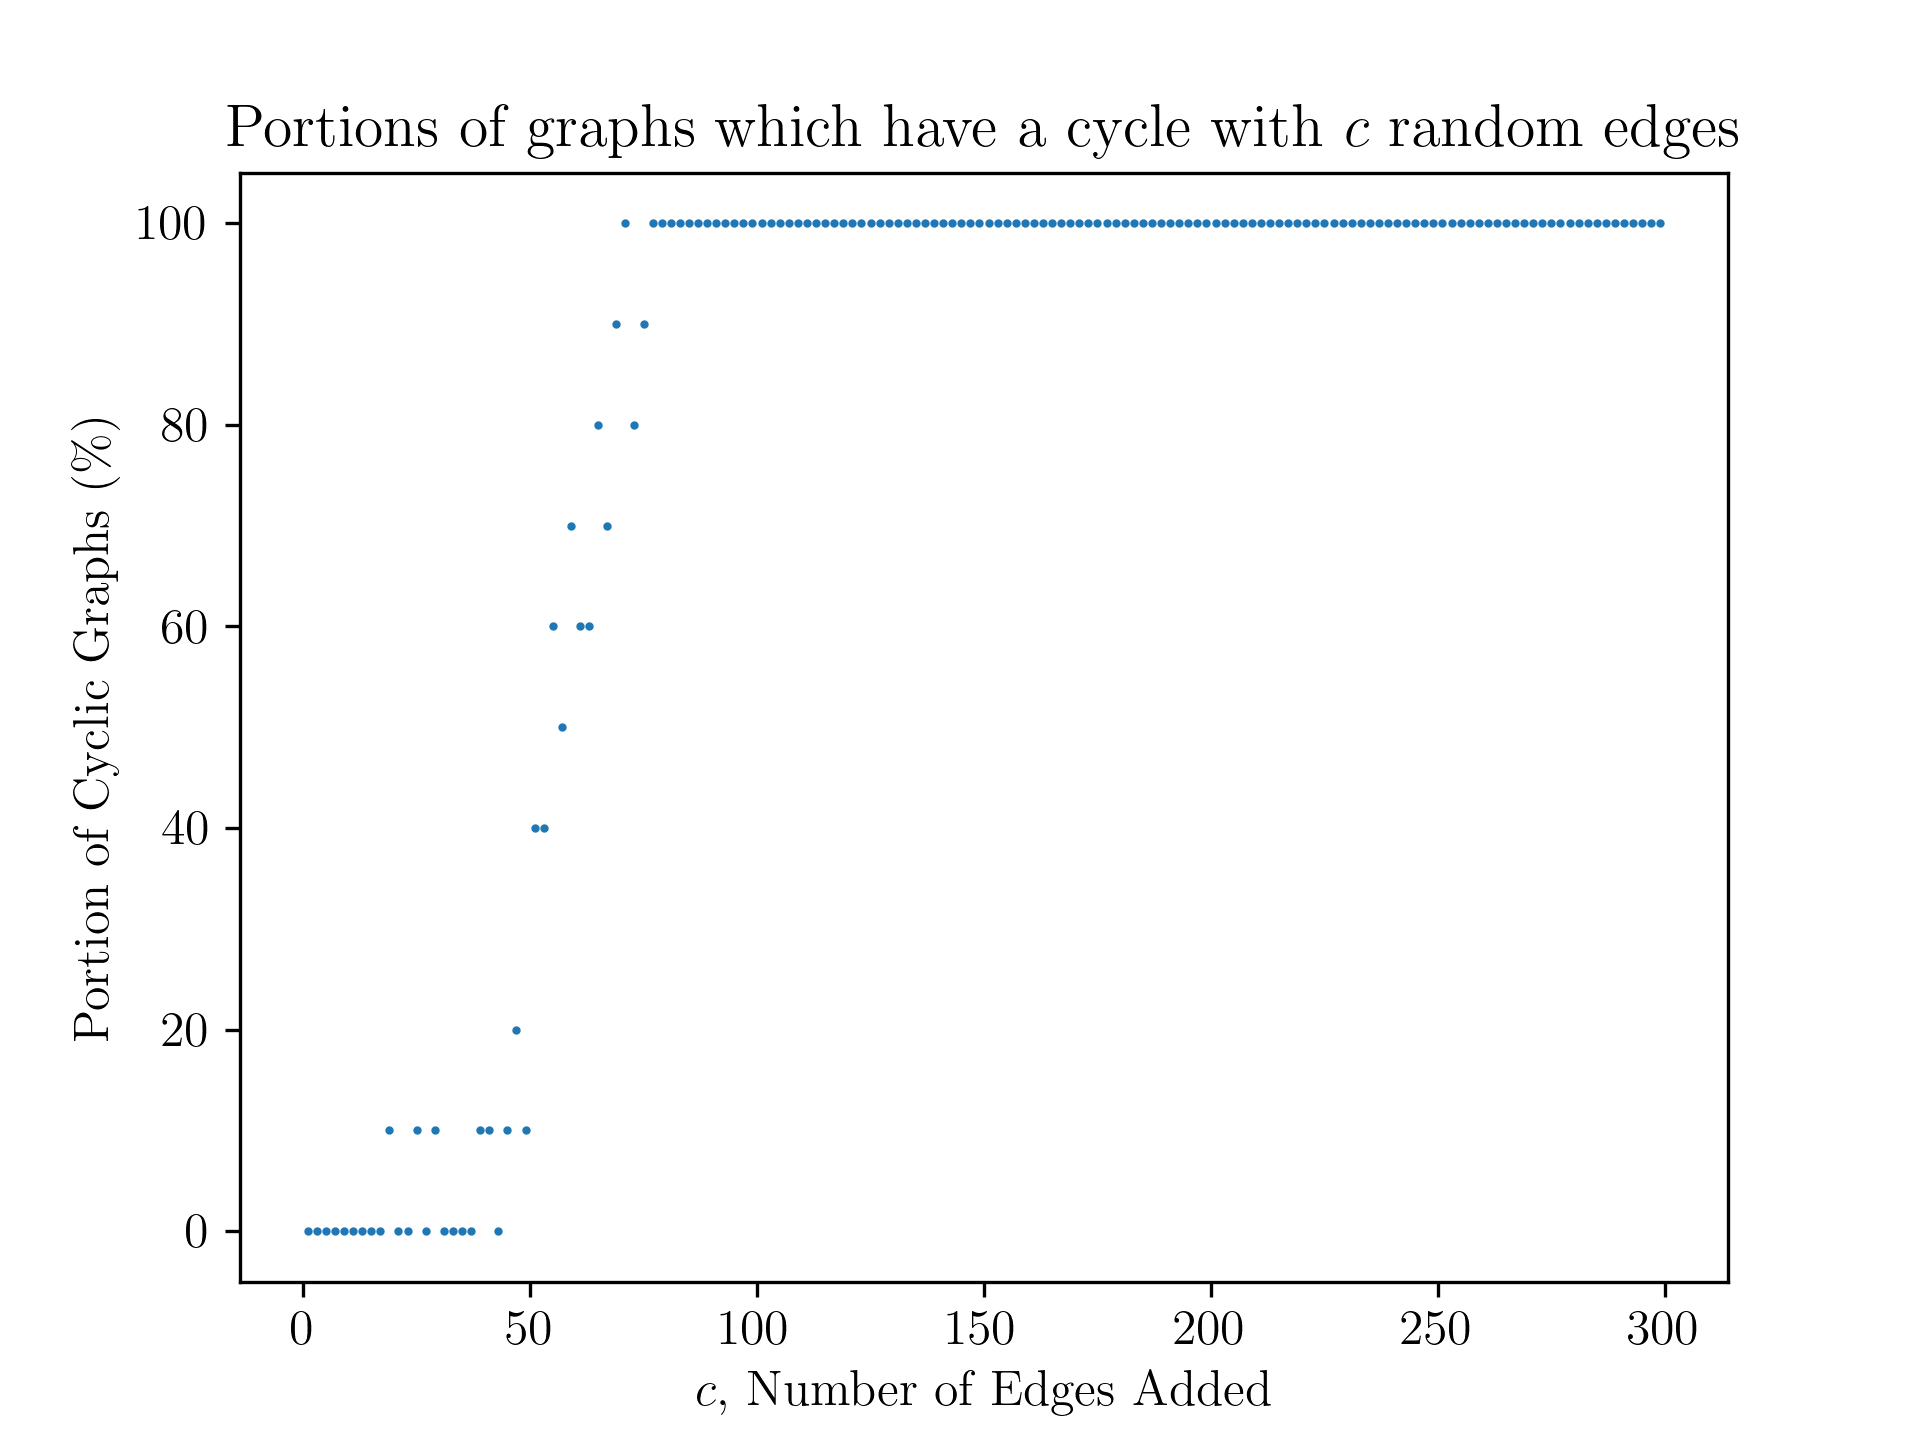
\includegraphics[width=0.8\linewidth]{cyclic}
  \caption{Cyclic portion vs. \(c\)}
  \label{fig:cyclic}
\end{figure}
\begin{figure}[h]
  \centering
  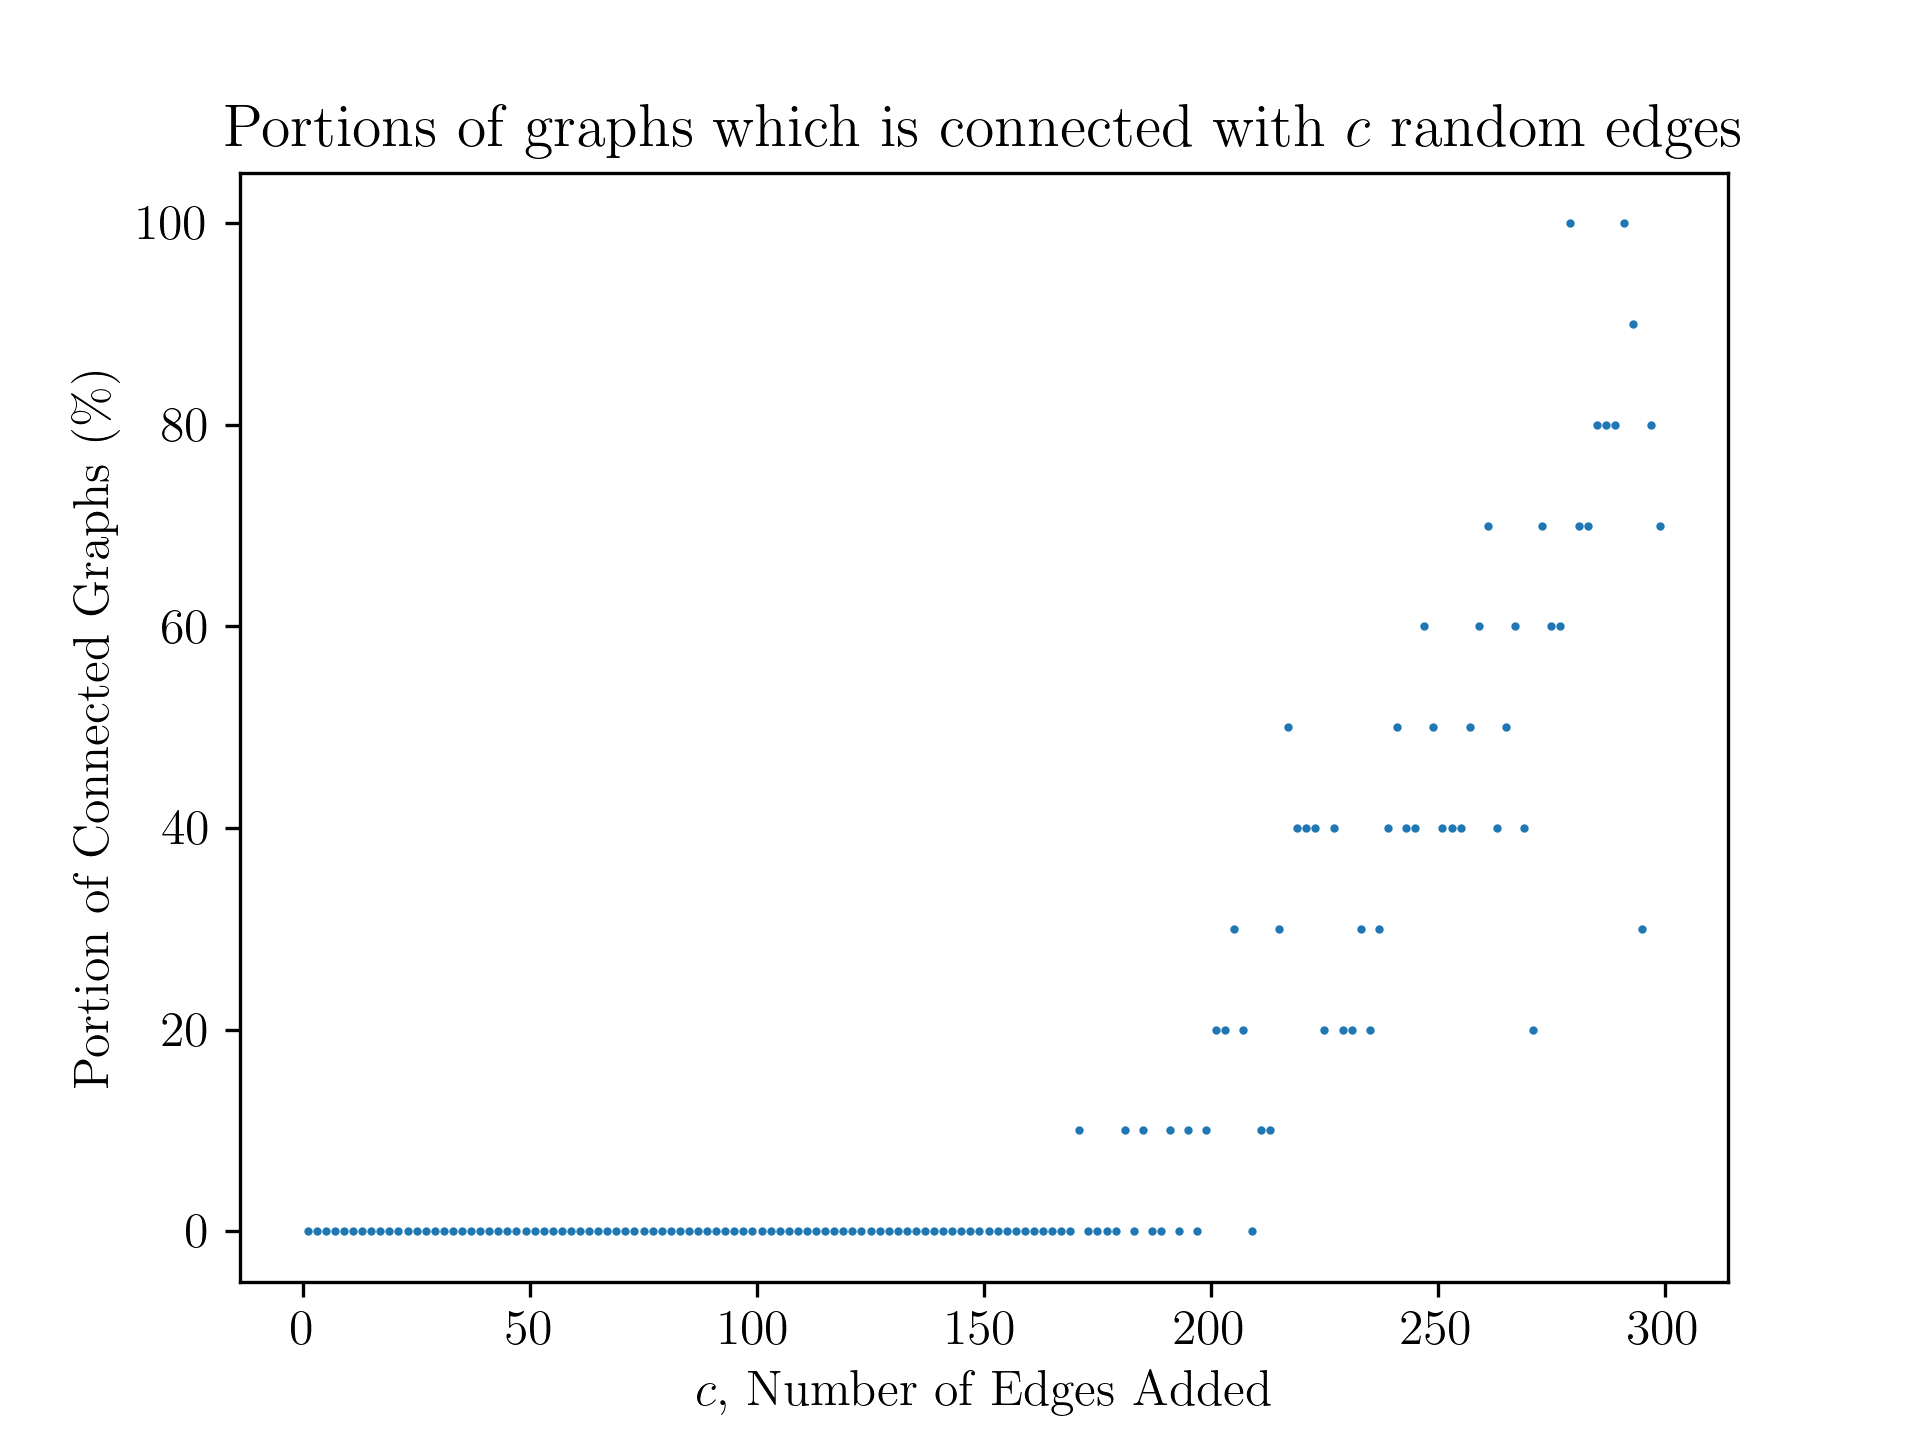
\includegraphics[width=0.8\linewidth]{connect}
  \caption{Connected portion vs. \(c\)}
  \label{fig:connect}
\end{figure}

\end{document}